% This is samplepaper.tex, a sample chapter demonstrating the
% LLNCS macro package for Springer Computer Science proceedings;
% Version 2.20 of 2017/10/04
%
\documentclass[runningheads]{llncs}
%
\usepackage{graphicx,subfig}
\usepackage{amstext,amsmath,amssymb,bm,bbm,mathtools}
\usepackage[export]{adjustbox}

\newtheorem{ddef}{Definition}
\DeclareMathOperator*{\argmin}{arg\,min}
\DeclarePairedDelimiter\norm{\lVert}{\rVert}%
\DeclarePairedDelimiter\abs{\lvert}{\rvert}%

% Used for displaying a sample figure. If possible, figure files should
% be included in EPS format.
%
% If you use the hyperref package, please uncomment the following line
% to display URLs in blue roman font according to Springer's eBook style:
% \renewcommand\UrlFont{\color{blue}\rmfamily}

\begin{document}
%
\title{Digital Curvature Evolution Model for Image Segmentation\thanks{This  work has  been  partly  funded by CoMeDiC ANR-15-CE40-0006 research grant.}}

\author{Daniel Antunes\inst{1}
Jacques-Olivier Lachaud\inst{1}
Hugues Talbot\inst{2}}
%
\authorrunning{D. Antunes et al.}
% First names are abbreviated in the running head.
% If there are more than two authors, 'et al.' is used.
%
\institute{Universit{\'e} Savoie Mont Blanc, LAMA, UMR CNRS 5127, F-73376, France
\email{daniel.martins-antunes, jacques-olivier.lachaud@univ-savoie.fr} \and
CentraleSupelec Universit\'e Paris-Saclay, \'equipe INRIA GALEN\\
\email{hugues.talbot@centralesupelec.fr}}
%
\maketitle              % typeset the header of the contribution
%
\begin{abstract}
  Recent works have indicated the potential of using curvature as a
  regularizer in image segmentation, in particular for the class of
  thin and elongated objects. These are ubiquitous in biomedical
  imaging (e.g. vascular networks), in which length regularization can
  sometime perform badly, as well as in texture
  identification. However, curvature is a second-order differential measure,
  and so its estimators are sensitive to noise. The straightforward
  extensions to Total Variation are not convex, making them a challenge
  to optimize.  State-of-art techniques make use of a coarse
  approximation of curvature that limits practical applications.

  We argue that curvature must instead be computed using a multigrid
  convergent estimator, and we propose in this paper a new digital
  curvature flow which mimics continuous curvature flow. We
  illustrate its potential as a post-processing step to a variational
  segmentation framework.
 
\keywords{Multigrid convergence  \and Digital estimator \and Curvature \and Shape Optimization \and Image Segmentation.}
\end{abstract}
%
%
%
\setcounter{footnote}{0}
\section{Introduction}

Geometric quantities are particularly useful as regularizers, especially when some prior information about the object
geometry is known. Length penalization is a general purpose regularizer and the literature is vast on models
that make use of it \cite{casseles97,appleton05}. However, this regularizer shows its limitations when segmenting thin
and elongated objects, as it tends to return disconnected solutions. Such drawback can sometime be overcome by injecting
curvature regularization \cite{zehiry10}.
				
One of the first successful uses of curvature in image processing is the inpainting algorithm described in
\cite{masnou98}. The authors evaluate the elastica energy along the level lines of a simply-connected image to
reconstruct its occluded parts. The non-intersection property of level lines allows the construction of an efficient
dynamic programming algorithm. Nonetheless, it is still a challenging task to inject curvature in the context of image
segmentation.

The state-of-art methods are difficult to optimize and not scalable \cite{zehiry10,schoenemann09,nieuwenhuis14}. In
order to achieve reasonable running times, such approaches make use of coarse curvature estimations for which the approximation
error is unknown. Improving the quality of the curvature estimator has an important impact on the accuracy of the
results, but is computationally too costly in these methods. Recently, new multigrid convergent estimators for curvature
have been proposed \cite{schindele17,coeurjolly13,roussillon11}, motivating us to search for models in which they can be
applied.

In this work, we investigate the use of a more suitable curvature estimator with multigrid convergent property and its
application as a boundary regularizer in a digital flow minimizing its squared curvature. Our method decreases the
elastica energy of the contour and its evolution is evaluated on several digital flows. Finally, we present an
application of the model as a post-processing step in a segmentation framework. The code is freely available on
github\footnote{https://www.github.com/danoan/BTools}.

\textit{Outline}. Section two reviews the concept of multigrid convergence and highlights its importance for the
definition of digital estimators. Next, we describe two convergent estimators used in this paper, one for tangent and
the other for curvature. They are used in the optimization model and in the definition of the digital elastica. Section
three describes the proposed curvature evolution model along with several illustrations of digital flows. Section four
explains how to use the evolution model as a post-processing step in an image segmentation framework. Finally, sections
five and six discuss the results and point directions for future work.




\section{Multigrid Convergent Estimators}



A digital image is the result of some quantization process over an object $X$ lying in some continuous space of
dimension $2$ (here).  For example, the Gauss digitization of $X$ with grid step $h>0$ is defined as
\begin{align*}
	D_h(X) = X \cap (h\mathbb{Z})^2.
\end{align*} 

Given an object $X$ and its digitization $D_h(X)$, a digital estimator $\hat{u}$ for some geometric quantity $u$ is
intended to compute $u(X)$ by using only the digitization. This problem is not well-posed, as the same digital object
could be the digitization of infinitely many objects very different from $X$. Therefore, a characterization of what constitutes
a good estimator is necessary.

Let $u$ be some geometric quantity of $X$ (e.g. tangent, curvature). We wish to devise a digital estimator $\hat{u}$ for
$u$. It is reasonable to state that $\hat{u}$ is a good estimator if $\hat{u}(D_h(X))$ converges to $u(X)$ as we refine
our grid. For example, counting pixels is a convergent estimator for area (with a rescale of $h^2$); but counting
boundary pixels (with a rescale of $h$) is not a convergent estimator for perimeter. Multigrid convergence is the
mathematical tool that makes this definition precise. Given any subset $Z$ of $(h\mathbb{Z})^2$, we can represent it as a
union of axis-aligned squares with edge length $h$ centered on the point of $Z$. The topological boundary of this union
of cubes is called {\em $h$-frontier} of $Z$. When $Z=D_h(X)$, we call it {\em $h$-boundary of $X$} and denote it by
$\partial_h X$.
%% In the following, let the $h$-frontier of $D_h(X)$ to be defined as $\partial D_h(X) = \partial \left( \frac{1}{h} \cdot X \right) \cap \mathbb{Z}^2$.

\begin{ddef}[Multigrid convergence for local geometric quantites]
  A local discrete geometric estimator $\hat{u}$ of some geometric
  quantity $u$ is (uniformly) multigrid convergent for the family $\mathbb{X}$ if
  and only if, for any $X \in \mathbb{X}$, there exists a grid step
  $h_X>0$ such that the estimate $\hat{u}(D_h(X),\hat{x},h)$ is
  defined for all $\hat{x} \in \partial_hX$ with $ 0 < h < h_X$, and
  for any $x \in \partial X$,
  \begin{equation*}
    \forall \hat{x} \in  \partial_hX \text{ with } \norm{ \hat{x} - x }_{\infty} \leq h, \norm{ \hat{u}(D_h(X),\hat{x},h) - u(X,x)} \leq \tau_{X}(h),			
  \end{equation*}
  where $\tau_{X}:\mathbb{R}^{+}\setminus\{0\} \rightarrow
  \mathbb{R}^{+}$ has null limit at $0$. This function defines the
  speed of convergence of $\hat{u}$ towards $u$ for $X$.
\end{ddef}
	
For a global geometric quantity (e.g. perimeter, area, volume), the definition remains the same, except that the mapping
between $\partial X$ and $\partial_h X$ is no longer necessary.
	
Multigrid convergent estimators provide a quality guaranty and should be preferred over non-multigrid convergent
ones. In the next section, we describe two estimators that are important for our purpose.

\subsection{Tangent and Perimeter Estimators}

The literature presents several perimeter estimators that are multigrid convergent (see
\cite{coeurjolly04,coeurjolly12} for a review), but in order to define the digital elastica we need a local estimation
of length and we wish that integration over these local length elements gives a multigrid convergent estimator for the
perimeter.

\begin{ddef}[Elementary Length]
  Let a digital curve $C$ be represented as a sequence of grid vertices in a grid cell representation of digital objects (in grid with step $h$). Further, let $\hat{\theta}$ be a multigrid convergent estimator for tangent. The elementary length $\hat{s}(e)$ at some grid edge $e\in C$ is defined as
  \begin{align*}
    \hat{s}(e) = h \cdot \hat{\theta}(l) \cdot or(e),
  \end{align*}
  where $or(e)$ denotes the grid edge orientation.
\end{ddef}
The integration of the elementary length along the digital curve is a multigrid convergent estimator for perimeter if
one uses the $\lambda$-MST \cite{lachaud07} tangent estimator (see \cite{lachaud06}).



%We represent a curve as a sequence of pointels (zero dimensional elements of the digital grid. Its respective higher dimensional counterparts are called linels and pixels). Sequence indexes are recovered by function $i_C(\cdot)$. The curve segment $C_{p,q}$ between pointels $p,q$ is a digital straight segment (DSS) if $C_{p,q}$ is a standard line.
%
%
%\begin{ddef}[Standard line] 
%The set of points
%$(x, y)$ of the digital plane verifying $\mu \leq ax -by \leq \abs{a} + \abs{b}$ , with $a,b$ and $\mu$
%integer numbers, is called the standard line
%with slope $a/b$ and shift $\mu$.
%\end{ddef}
%
%The $\lambda$-MST estimates the tangent of some curve $C$ at some pointel $p$ as a ponderated sum over the set of maximal digital straight segments of $C$ containing $p$.
%
%
%
%The curve $C$ can be covered by its set of maximal DSS $\mathcal{S}$. Hence, every pointel belongs to at least one maximal DSS. In fact, a pointel $p$ can be present in two or more elements of $\mathcal{S}$. We denote the pencil of $p$ by $\mathcal{P}(p) \subset \mathcal{S}$ as the set of maximal DSS which passes through $p$. We are now ready to characterize the eccentricity between a pointel $p$ and its pencil elements $M \in \mathcal{P}(p)$.
%
%\begin{align*}
%	e_p(M) = \frac{\abs{i_M(p) - i_M(q)} }{\abs{M}}. 
%\end{align*}
%
%The eccentricity is used to define the weight function $\lambda:[0,1]\rightarrow \mathbb{R}^+$. A good choice would be bell-shaped functions as the $C^2$ function $64(-x^6 + 3x^5 - 3x^4 + x^3)$ or the $C^{\infty}$ function $exp(4 - \frac{1}{x} - \frac{1}{1-x}).$ as noted by \cite{lachaud07}.
%
%\begin{ddef}[$\lambda$-MST] 
%The $\lambda$-maximal segment tangent direction at pointel $p$ is then defined as the weighted combination of the directions of the surrounding maximal segments:
%\end{ddef}
%
%\begin{align*}
%	\hat{\theta}(p) = \frac{ \sum_{M \in \mathcal{P}}{\lambda( e_p(M) )}\theta_M }{\sum_{M \in \mathcal{P}}{\lambda( e_p(M) )}}.
%\end{align*}
%
%The $\lambda$-MST is linearly convergent with average rate $O(h^{\frac{1}{3}})$ for the class of convex shapes with bounded curvature and finite number of inflexion points. A multigrid convergent estimator for length with equal convergence properties can be derived by integration.
%
%\begin{align*}
%	\hat{s} = h \cdot \sum_{l \in \mathcal{L}(C)}{\hat{\theta}(l) \cdot or(l)},
%\end{align*}
%
%where $\mathcal{L}(C)$ is the linel set of $C$ and $or(\cdot)$ the direction of a linel.


\subsection{Integral Invariant Curvature Estimator}
Generally, an invariant $\sigma$ is a real-valued function from some space $\Omega$ which value is unaffected by the action
of some group $\mathfrak{G}$ on the elements of the domain
\begin{align*}
  x \in \Omega, g \in \mathfrak{G}, \sigma(x) = v \longleftrightarrow \sigma(g \cdot x ) = v.
\end{align*}
Perimeter and curvature are examples of invariants for shapes on $\mathbb{R}^2$ with respect to the euclidean group
(rigid transformations). Definition of integral area invariant and its one-to-one correspondence with curvature is
proven in \cite{manay04}.


\begin{ddef}[Integral area invariant]
  Let $X \subset \mathbb{R}^2$ and $B_r(p)$ the ball of radius $r$ centered at point $p$. Further, let
  $\mathbbm{1}_X(\cdot)$ be the characteristic function of $X$. The integral area invariant $\sigma_{X,r}(\cdot)$ is
  defined as
  \begin{align*}
    \forall p \in \partial X, \quad \sigma_{X,r}(p) = \int_{B_r(p)}{ \mathbbm{1}_X(x) dx}.
  \end{align*}
\end{ddef}


The value $\sigma_{X,r}(p)$ is the intersection area of ball $B_r(p)$ with shape $X$. By locally approximating the shape
at point $p \in X$, one can rewrite the intersection area $\sigma_{X,r}(p)$ in the form of the Taylor expansion
\cite{pottman09}
	
\begin{align*}
  \sigma_{X,r}(p) = \frac{\pi}{2}r^2 - \frac{\kappa(X,p)}{3}r^3 + O(r^4),
\end{align*}
		
where $\kappa(X,p)$ is the curvature of $X$ at point $p$. By isolating $\kappa$ we can define a curvature estimator
	
\begin{align}
  \tilde{\kappa}(p) \coloneqq \frac{3}{r^3}\left( \frac{\pi r^2}{2} - \sigma_{X,r}(p) \right),
  \label{eq:curvature_approximation}
\end{align}
	
Such an approximation is convenient as one can simply devise a multigrid convergent estimator for the area.

\begin{ddef}	
  Given a digital shape $D \subset (h \mathbb{Z})^2$, a multigrid convergent estimator for the area $\widehat{Area}(D,h)$ is defined as	
		
  \begin{align}
    \widehat{Area}(D,h) \coloneqq h^2\text{Card}\left( D \right).	
    \label{eq:digital_estimator_area}
  \end{align}
\end{ddef}
	
In \cite{coeurjolly13}, the authors combine the approximation\eqref{eq:curvature_approximation} and digital estimator
\eqref{eq:digital_estimator_area} to define a multigrid convergent estimator for the curvature.

\begin{ddef}[Integral Invariant Curvature Estimator]
  Let $D \subset (h \mathbb{Z})^2$ a digital shape. The integral invariant curvature estimator is defined as
  \begin{align*}
    \hat{\kappa}_{r}(D,x,h) \coloneqq \frac{3}{r^3} \left( \frac{\pi r^2}{2} - \widehat{Area} \left( B_{r} ( x ) \cap D, h \right) \right).
    %% \hat{\kappa}_{r}(D,x,h) \coloneqq \frac{3}{r^3} \left( \frac{\pi r^2}{2} - \widehat{Area} \left( B_{r/h} ( \frac{1}{h} \cdot x ) \cap D, h \right) \right).
  \end{align*}
\end{ddef}


This estimator is robust to noise and can be extended to estimate the mean curvature of three dimensional shapes.


\section{Digital Curvature Evolution Model}


Our goal is to deform a digital object in order to minimize the elastica energy along its contour. Our strategy is to
define the digital elastica by using the elementary length and the integral invariant curvature estimators and minimize
its underlying binary energy. However, the derived energy is of order four and difficult to optimize. Therefore we
propose an indirect method to minimize it. %This method can be interpreted as a gradient flow of the elastica energy,
%even though it is entirely defined in discrete terms.


\subsection{Ideal Global Optimization Model}

We evaluate the quality of a boundary by evaluating the elastica energy along it. Let $\kappa (\cdot)$ denote the curvature function evaluated on the contour of some shape $X$. In continuous terms, the elastica energy is defined as 
\begin{align*}
  E(X) = \int_{\partial X}{(\alpha + \beta \kappa^2) ds}, \quad \text{for~} \alpha \ge 0, \beta \ge 0.
\end{align*}

We are going to use the digital version of the energy, using multigrid convergent estimators. The energy, in this case, is also multigrid convergent.
\begin{align}
	\hat{E}( D_h(X) ) = \sum_{x \in \partial D_h(X)}{ \hat{s}(x)\left(\; \alpha + \beta \hat{\kappa}_{r}^2(D_h(X),x,h) \; \right)}, 
	\label{eq:digital-energy}
\end{align}
where $\partial D_h(X)$ denotes the $4$-connected boundary of $D_h(X)$. In the following we omit the grid step $h$ to simplify expressions (or, putting it differently, we assume that $X$ is rescaled by $1/h$ and we set $h=1$).

A segmentation energy can be devised by including some data fidelity term $g$ in \eqref{eq:digital-energy}, but we need to restrict the optimization domain to consistent regions. We cannot properly estimate length and curvature along anything different from a boundary. Let $\Omega$ be the digital domain and $\mathcal{T}$ the family of subsets of $\Omega$ satisfying the property
\begin{align*}
	D \in \mathcal{T} \implies D \subset \Omega \text{ and } 4B(\partial D),
\end{align*} 
where $4B(\cdot)$ is the $4$-connected closed boundary predicate. 


For some $\gamma>0$, the segmented region $D^\star$ is defined as
\begin{align}
	D^{\star} = \argmin_{D \in \mathcal{T}}{\sum_{x \in \partial D}{ \hat{s}(x)\left(\; \alpha + \beta \hat{\kappa_{r}}^2(D,x) \; \right)} + \gamma \cdot g(D).}
	\label{eq:ideal_optimization_energy}
\end{align}

In its integer linear programming model \cite{schoenemann09}, Schoenemann restricts the optimization domain by imposing a set of constraints that enforces compact sets as solutions. However, the main difficulty here is the minimization of a third order binary energy. We are going to explore an alternative strategy.



\subsection{Nonzero Curvature Identification}

We can use the curvature estimator to detect regions of positive curvature. Given a digital object $D$ embedded in a domain $\Omega$, we define its pixel boundary set $P(D)$ as
\begin{align*}
	P(D) = \left\{ \: x \; | \; x \in D, |\mathcal{N}_4(x) \cap D|<4 \: \right\},
\end{align*}
where $\mathcal{N}_4(x)$ denotes the $4$-adjacent neighbor set of $x$ (without $x$). The following optimization regions are important in our process.

\[\arraycolsep=5pt
\begin{array}{rlr}
	O &= P(D) & \text{Optimization region.} \\
	F &= D - P(D) & \text{Trust foreground.} \\
	B &= \Omega - D & \text{Trust background.} \\
	A &= P(F) \cup P(B) & \text{Computation region}.
\end{array}
\]

Note that our definition of the optimization region guarantees that only connected solutions are produced. The computation region is defined around $O$ for symmetric issues. We proceed by minimizing the squared curvature energy along $A$ with respect to the optimization region $O$. 

\begin{align}			
	Y^{\star} = \argmin_{Y \in \{0,1\}^{|O|}} \sum_{p \in A}{\hat{\kappa}_{r}^2(p)}.
	\label{eq:curvature_highlighting_opt_problem}
\end{align}

We expand the squared curvature esimator for a single point $p \in A$ using \eqref{eq:curvature_approximation}. Define constants $c_1 = (3/r^3)^2$, $c_2=\pi r^2/2$. Hence,

\begin{align*}
\hat{\kappa}_{r}^2(p) &= c_1 \cdot \big(\: c_2 - \sigma_{D,r}(p) \: \big)^2 \\
&= c_1 \cdot \big(\: c_2^2 - 2c_2\sigma_{D,r}(p) + \sigma_{D,r}(p)^2 \: \big).
\end{align*}

Let $F_r(p) \subset F$ denote the intersection set between the estimating ball applied at $p$ with the foreground region. The subset $Y_r(p) \subset Y$ is defined  analogously. Substituting $\sigma_{D,r}(p) = |F_r(p)| + \sum_{y_i \in Y_r(p)}{y_i}$, we obtain

	\begin{align*}
		\hat{\kappa}_{r}^2(p) &= c_1 \cdot \left( \; c_2^2 - 2c_2 \cdot |F_r(p)| + |F_r(p)|^2 + 2\left( |F_r(p)| - c_2 \right) \cdot \sum_{y_i \in Y_r(p)}{y_i}  + \left( \sum_{y_i \in Y_r(p)}{y_i} \; \right) ^2 \right) \\[1em]
	\end{align*}
	
	Packing constants $C=c_2^2 - 2c_2 \cdot |F_r(p)| + |F_r(p)|^2$.
	
	\begin{align*}
		\hat{\kappa}_{r}^2(p) = c_1 \cdot \left( C + 2\left( |F_r(p)| - c_2 \right) \cdot \sum_{y_i \in Y_r(p)}{y_i} + \sum_{y_i \in Y_r(p)}{y_i^2} + 2 \cdot \sum_{ \substack{y_i,y_j \in Y_r(p) \\ i<j} }{y_iy_j}  \right)
	\end{align*}
	
	By ignoring constants and multiplication factors and using the binary character of the variables, problem \eqref{eq:curvature_highlighting_opt_problem} is equivalent to

	
\begin{align}			
	Y^{\star} = \argmin_{Y \in \{0,1\}^{|O|}} \sum_{p \in A}{ \left( { (1/2+ |F_r(p)|-c_2) \cdot \sum_{y_i \in Y_r(p)}{y_i} } + \sum_{ \substack{y_i,y_j \in Y_r(p) \\ i<j} }{y_iy_j} \right) }.
	\label{eq:curvature_highlighting_simplified}
\end{align}

Energy \eqref{eq:curvature_highlighting_simplified} is non-submodular, and minimizing it is a NP-Hard problem in the general case. The QPBOP \cite{rother07} method provides a partial labeling for the optimization variables with the property that all labeled variables belong to some optimal solution. However, some pixels may be left unlabeled. The optimization method is further discussed in section \ref{sec:optimization_method}. For $r=3$, evaluation of the model on a digital square produces figure \ref{fig:naive_solution}.


	\begin{figure}[!ht]
		\center
		\subfloat[\label{fig:naive_solution}]{%
		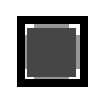
\includegraphics[scale=2.0]{images/qbo_1D_naive_solution_noneigh.eps}
		}%
		\hspace{40pt}
		\subfloat[\label{fig:naive_solution_updated}]{%
		
\includegraphics[scale=2.0]{images/qbo_1D_naive_solution_noneigh_updated.eps}}%
		\hspace{40pt}
		\subfloat[\label{fig:opt_regions}]{%

\includegraphics[scale=2.0]{images/opt-regions.eps}}%		
		\caption{Figure (a): White pixels denote variables labeled as one by QPBOP, while light gray pixels variables are labeled zero; Figure (b): Inverted labeling; Figure (c): Regions of interest: Background (black); Foreground (dark gray); Computation (light gray); and Optimization (white) regions.}	
					
	\end{figure}

        We interpret positive curvature at some point $p$ as a shortage of intersection points between the digital object
        and the estimating ball. The curvature can be reduced if the estimating ball is pulled towards the interior of the
        digital object, which is done by removing the highlighted pixels in figure \ref{fig:naive_solution}. In other words, the partial labeling is inverted, and unlabeled pixels remain unchanged. Points with
        negative curvature are detected similarly if we evaluate the model on the digital object complement.

\subsection{Digital Curvature Flow}

We derive the digital curvature flow by iteratively evaluating model \eqref{eq:curvature_highlighting_simplified} with a
slight modification. We extend the computation region to take into account more level sets ($\ell$) of the original object. As a
practical consequence, zones of high curvature are more likely to be detected, leading to a smaller number of unlabeled
pixels by QPBOP.

\begin{align*}
	A = \bigcup_{i\leq \ell}{ \partial F^{-i} \cup \partial B^{-i} },
\end{align*}
where the $-i$ exponent means an erosion by a square of side $i$. Figure \ref{fig:opt_regions} illustrates the different regions of the optimization model. 

At each flow step, the model is evaluated twice. In the second evaluation, we take care of concavities. The model is
executed on $\overline{D^{+1}}$, the complement of the dilation by a square of side one, and we swap foreground and
background regions. Figure \ref{fig:digital_flows} presents several digital curvature flows and table \ref{tab:digital_glows_elastica_result} lists the initial and final digital elastica energy for the tested shapes.

We observe that the choice of ball radius ($r$) and level sets ($\ell$) should take into account the image scale. For example, using a
radius that is too large might lead to a disconnected intersection zone and the accuracy of the estimator is compromised. This
explains the difference in flows in figure \ref{fig:digital_flows}. In practice, we observe that using a ball of radius
$3$ is sufficient to produce good results while achieving a reasonable running time.

\begin{figure}[!ht]
		\center
		\setcounter{subfigure}{-4}			
		\subfloat[$r=3,\ell=3$]{%
		\subfloat{%
		
\includegraphics[scale=0.025]{images/flow-b3-ls3/Ball.eps}
		}%
		\hspace{15pt}
		\subfloat{%
		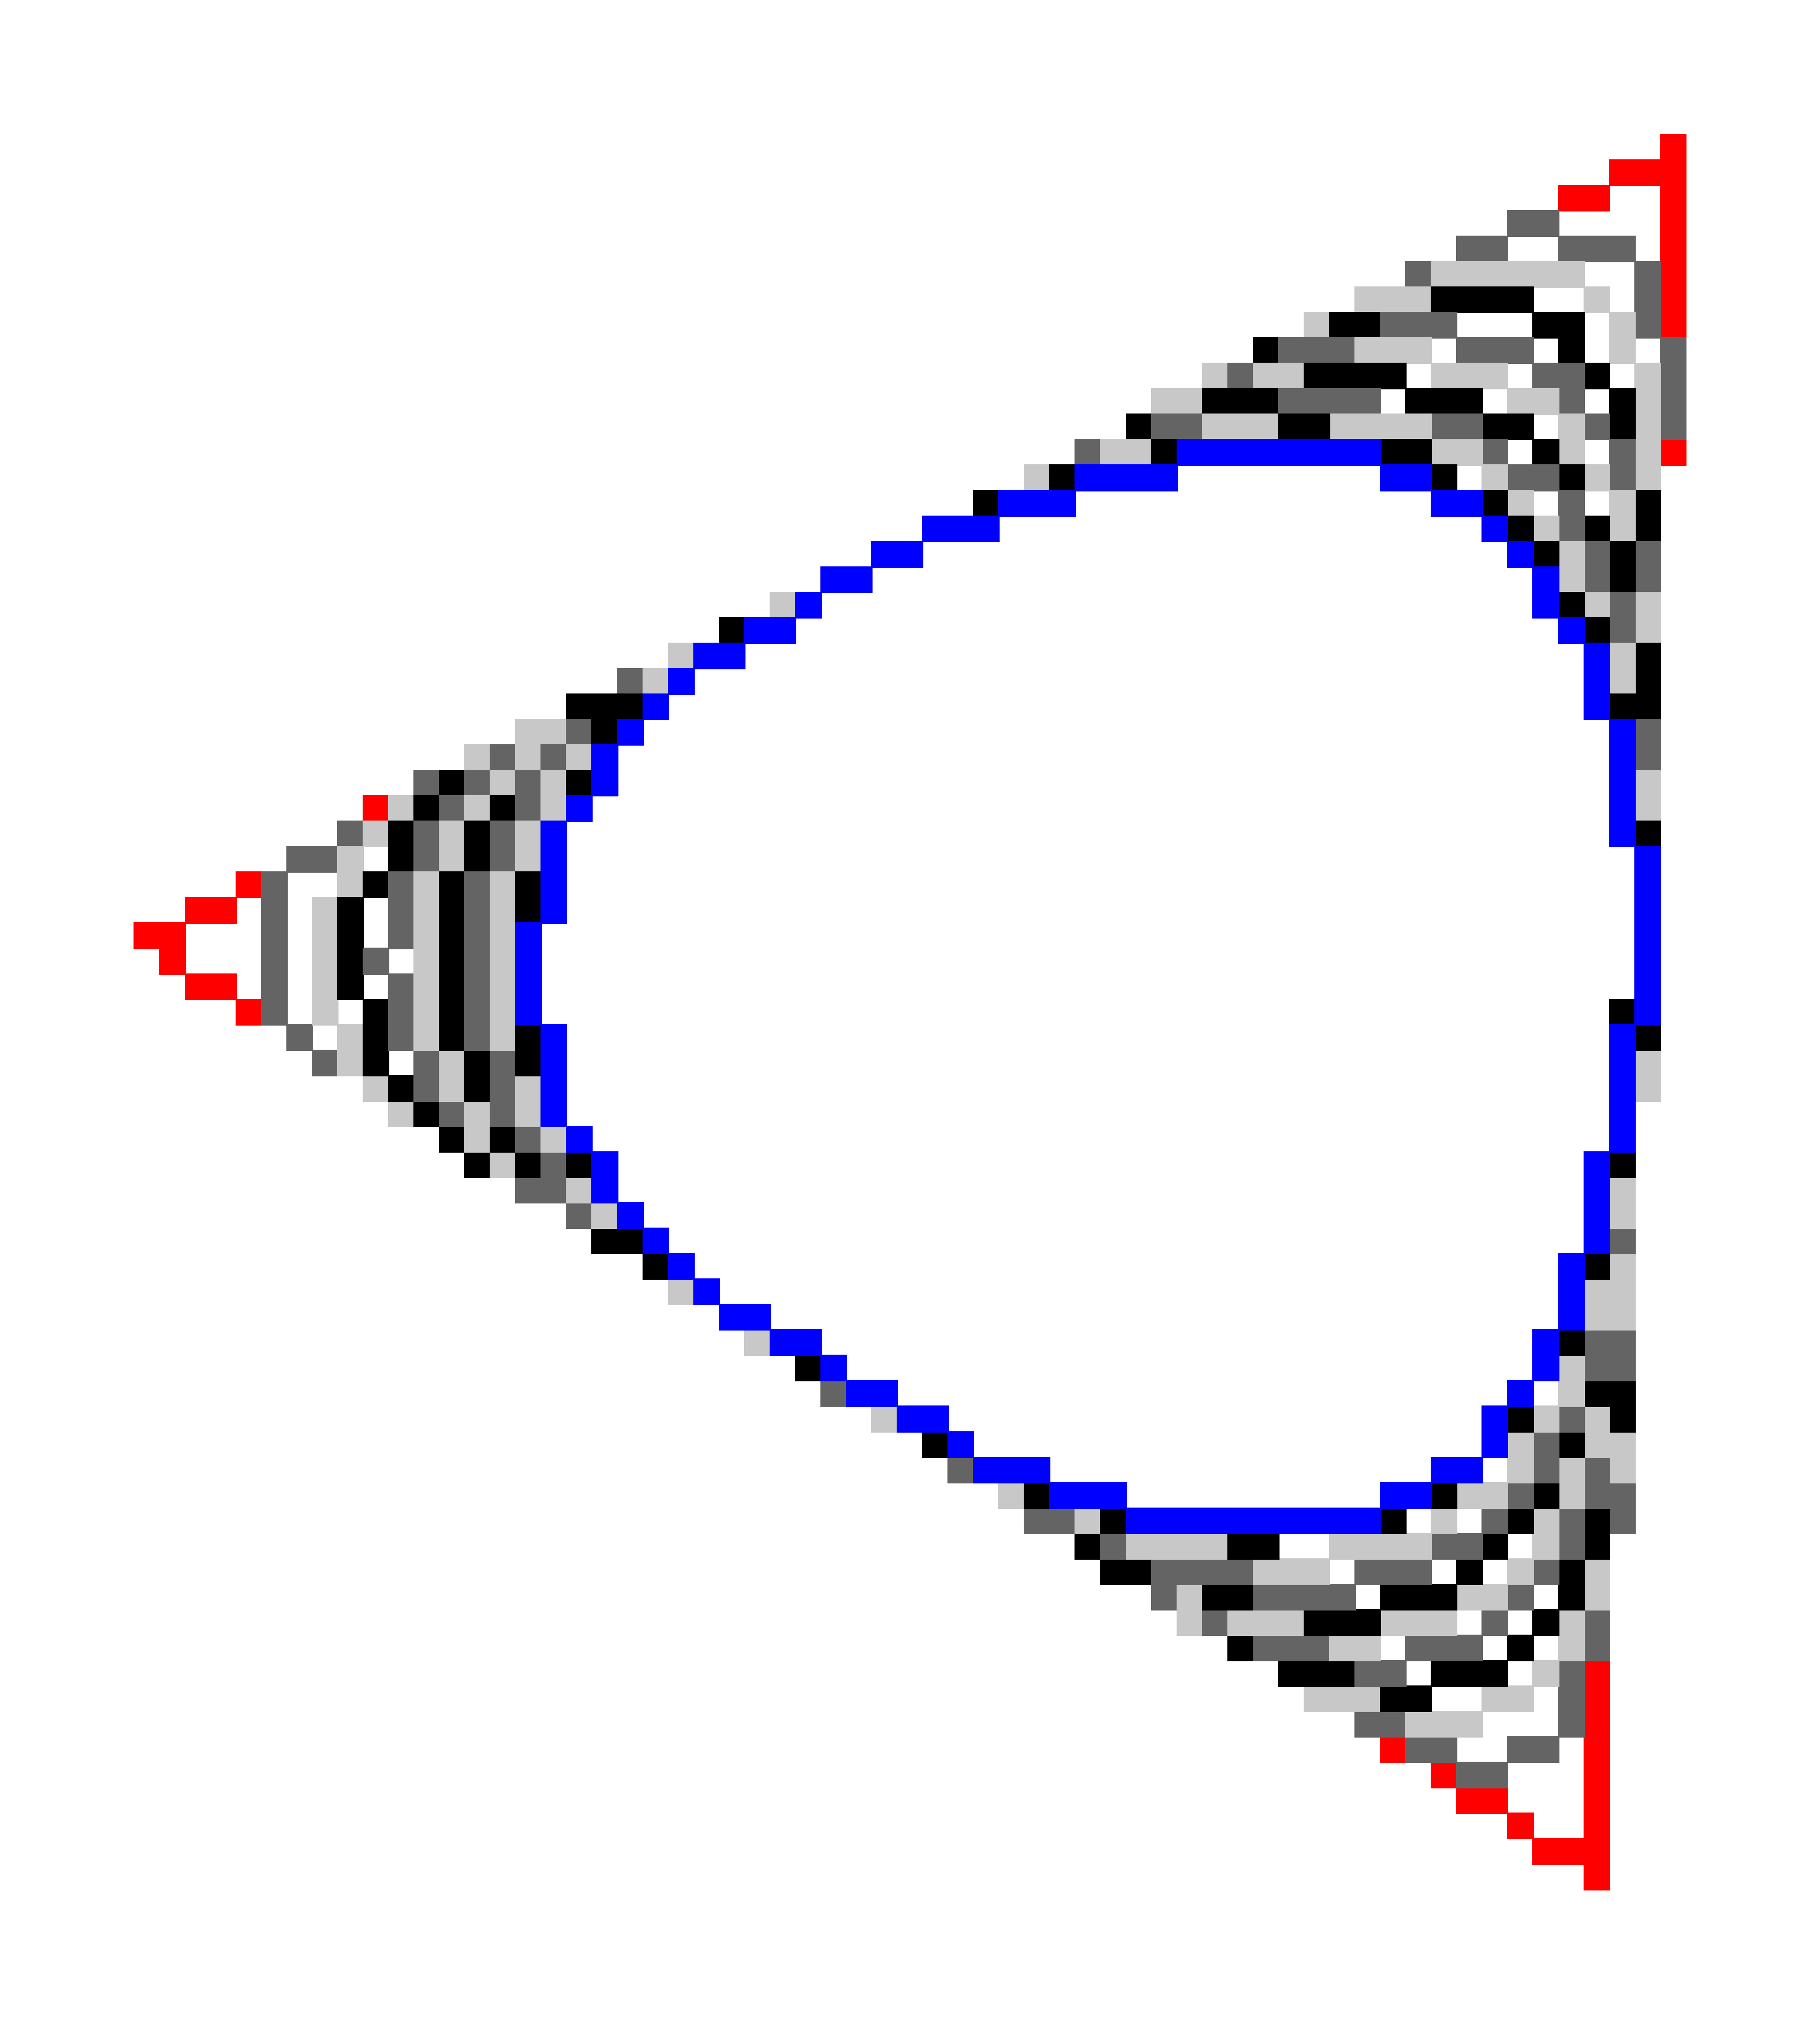
\includegraphics[scale=0.03]{images/flow-b3-ls3/Triangle.eps}}%
		\hspace{15pt}
		\subfloat{%

\includegraphics[scale=0.03]{images/flow-b3-ls3/Square.eps}}%		
		\hspace{15pt}	
		\subfloat{%

\includegraphics[scale=0.025]{images/flow-b3-ls3/Flower.eps}}%
		}

		\setcounter{subfigure}{-3}			
		\subfloat[$r=5,\ell=5$]{
		\subfloat{%
		
\includegraphics[scale=0.025]{images/flow-b5-ls5/Ball.eps}
		}%
		\hspace{15pt}
		\subfloat{%
		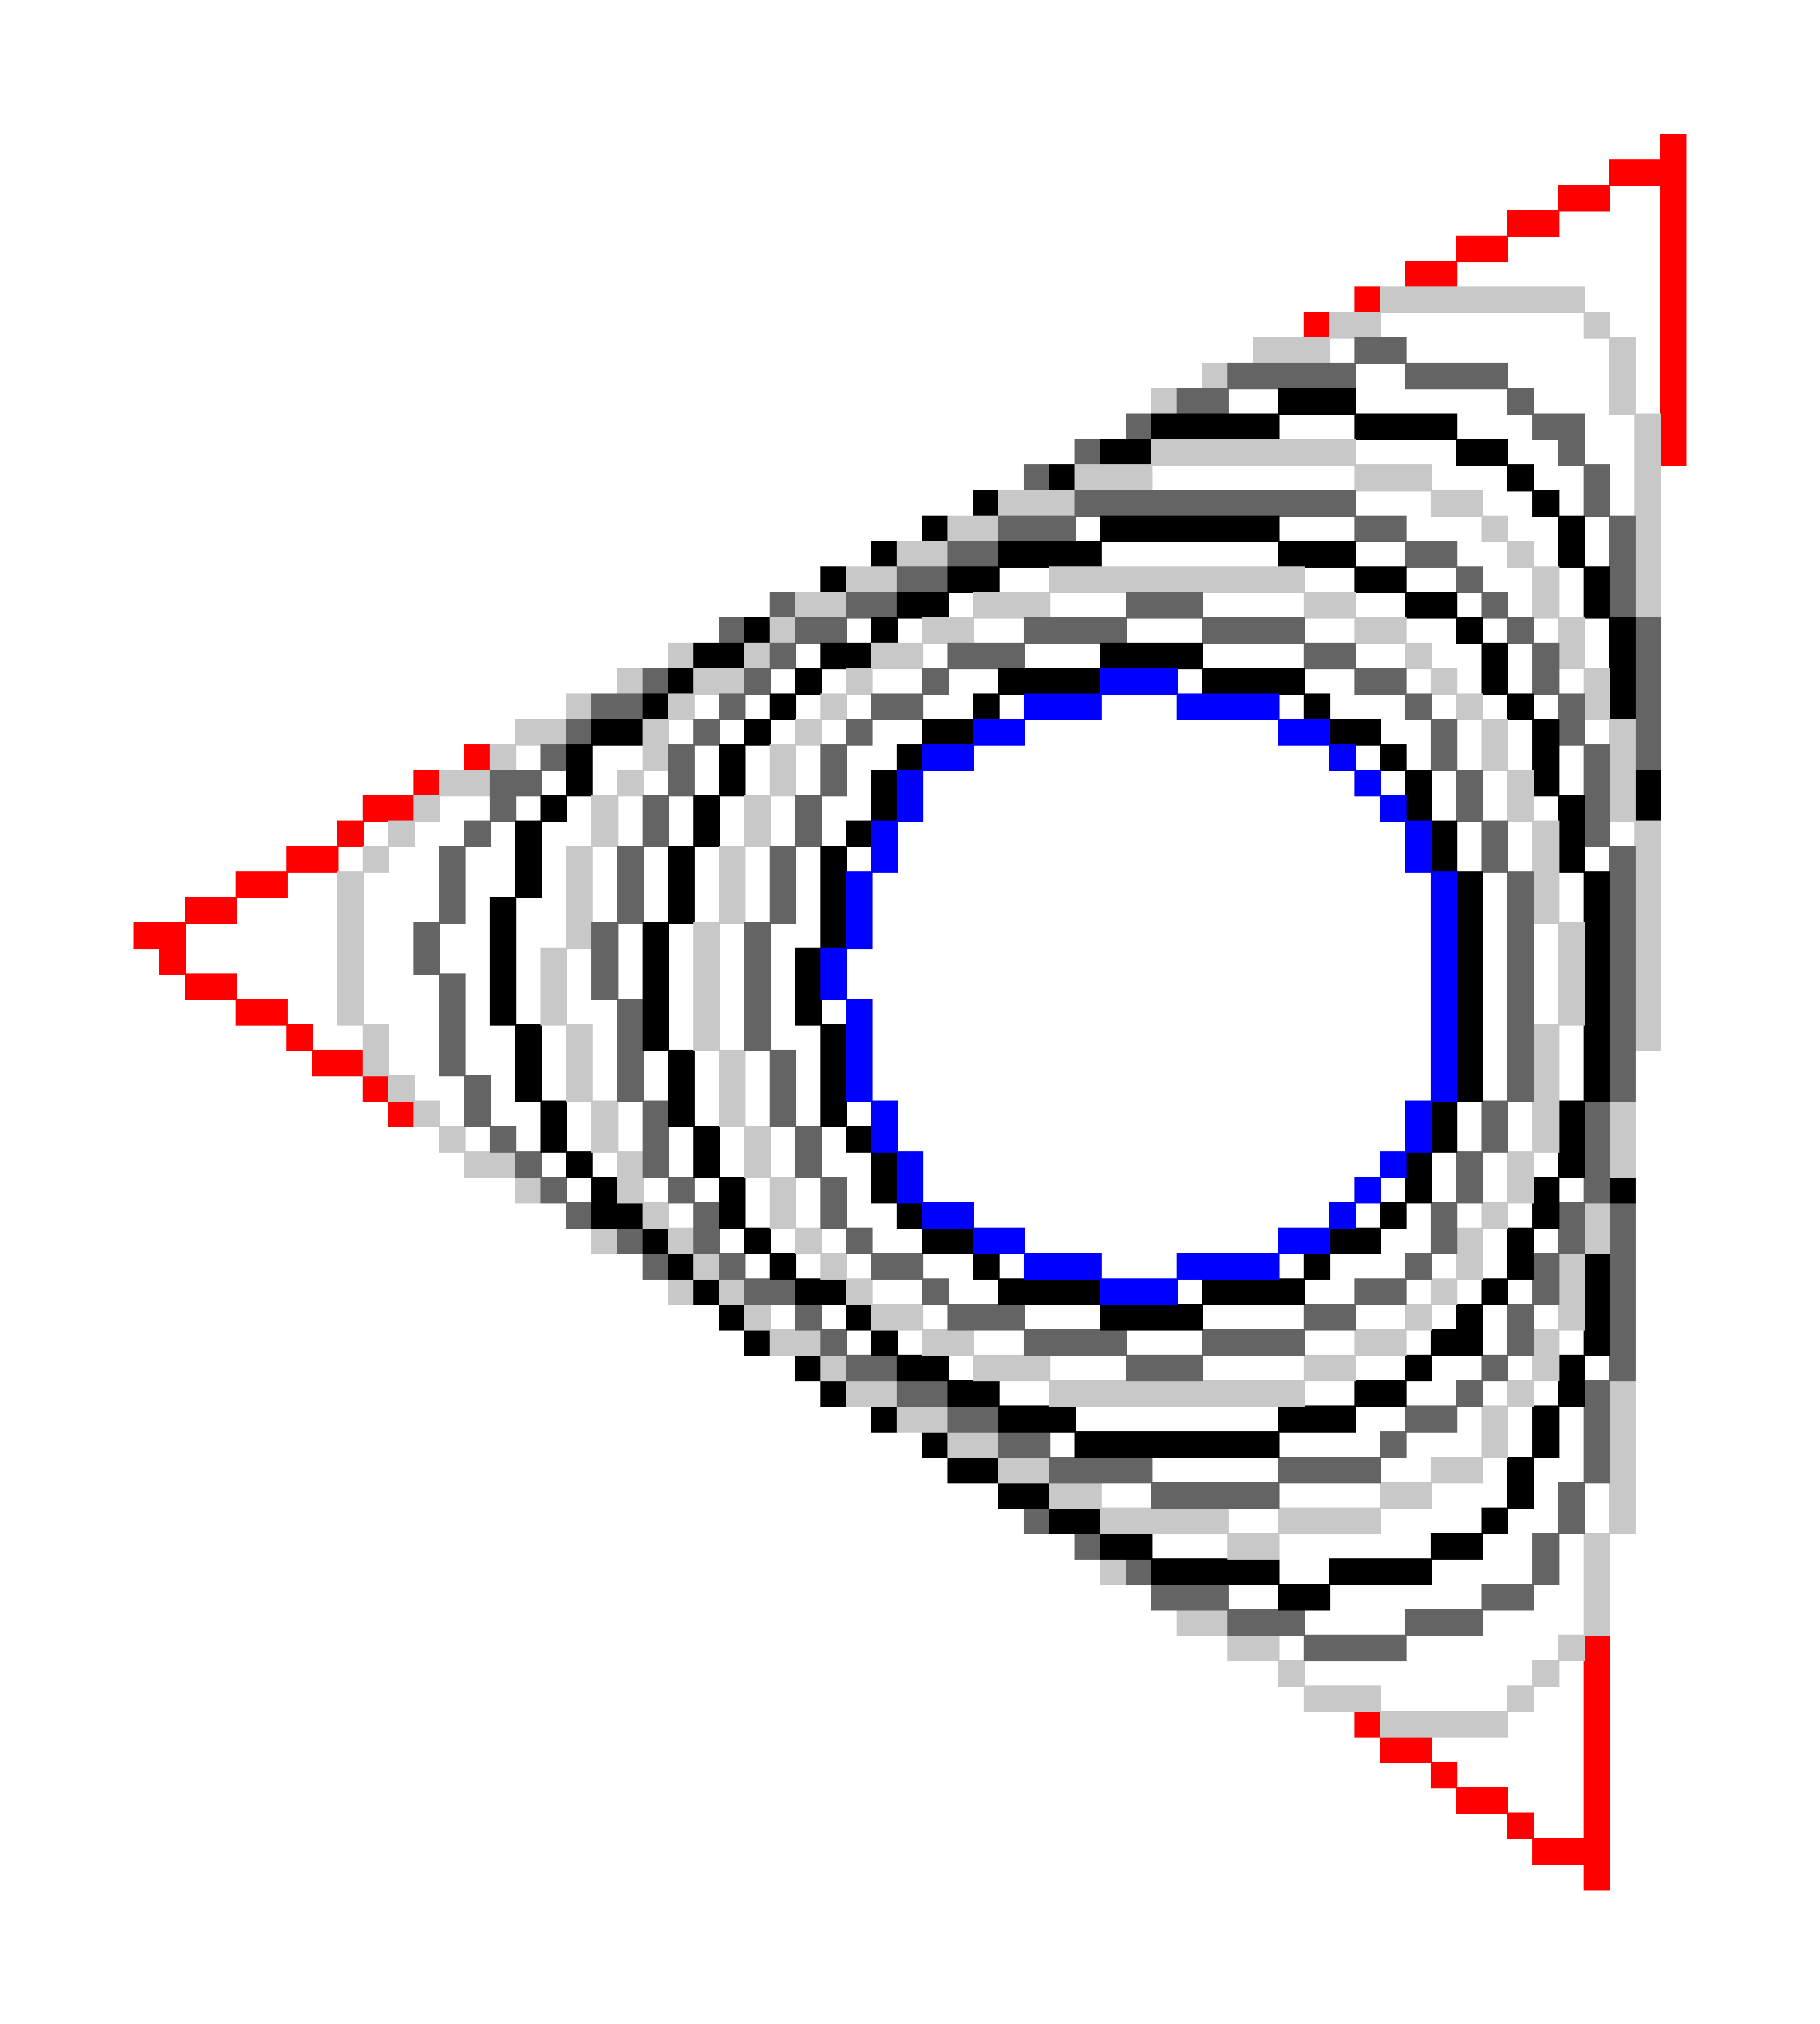
\includegraphics[scale=0.03]{images/flow-b5-ls5/Triangle.eps}}%
		\hspace{15pt}
		\subfloat{%

\includegraphics[scale=0.03]{images/flow-b5-ls5/Square.eps}}%		
		\hspace{15pt}
		\subfloat{%

\includegraphics[scale=0.025]{images/flow-b5-ls5/Flower.eps}}%
		}

		\setcounter{subfigure}{-2}			
		\subfloat[$r=10,\ell=10$]{
		\subfloat{%
		
\includegraphics[scale=0.025]{images/flow-b10-ls10/Ball.eps}
		}%
		\hspace{15pt}
		\subfloat{%
		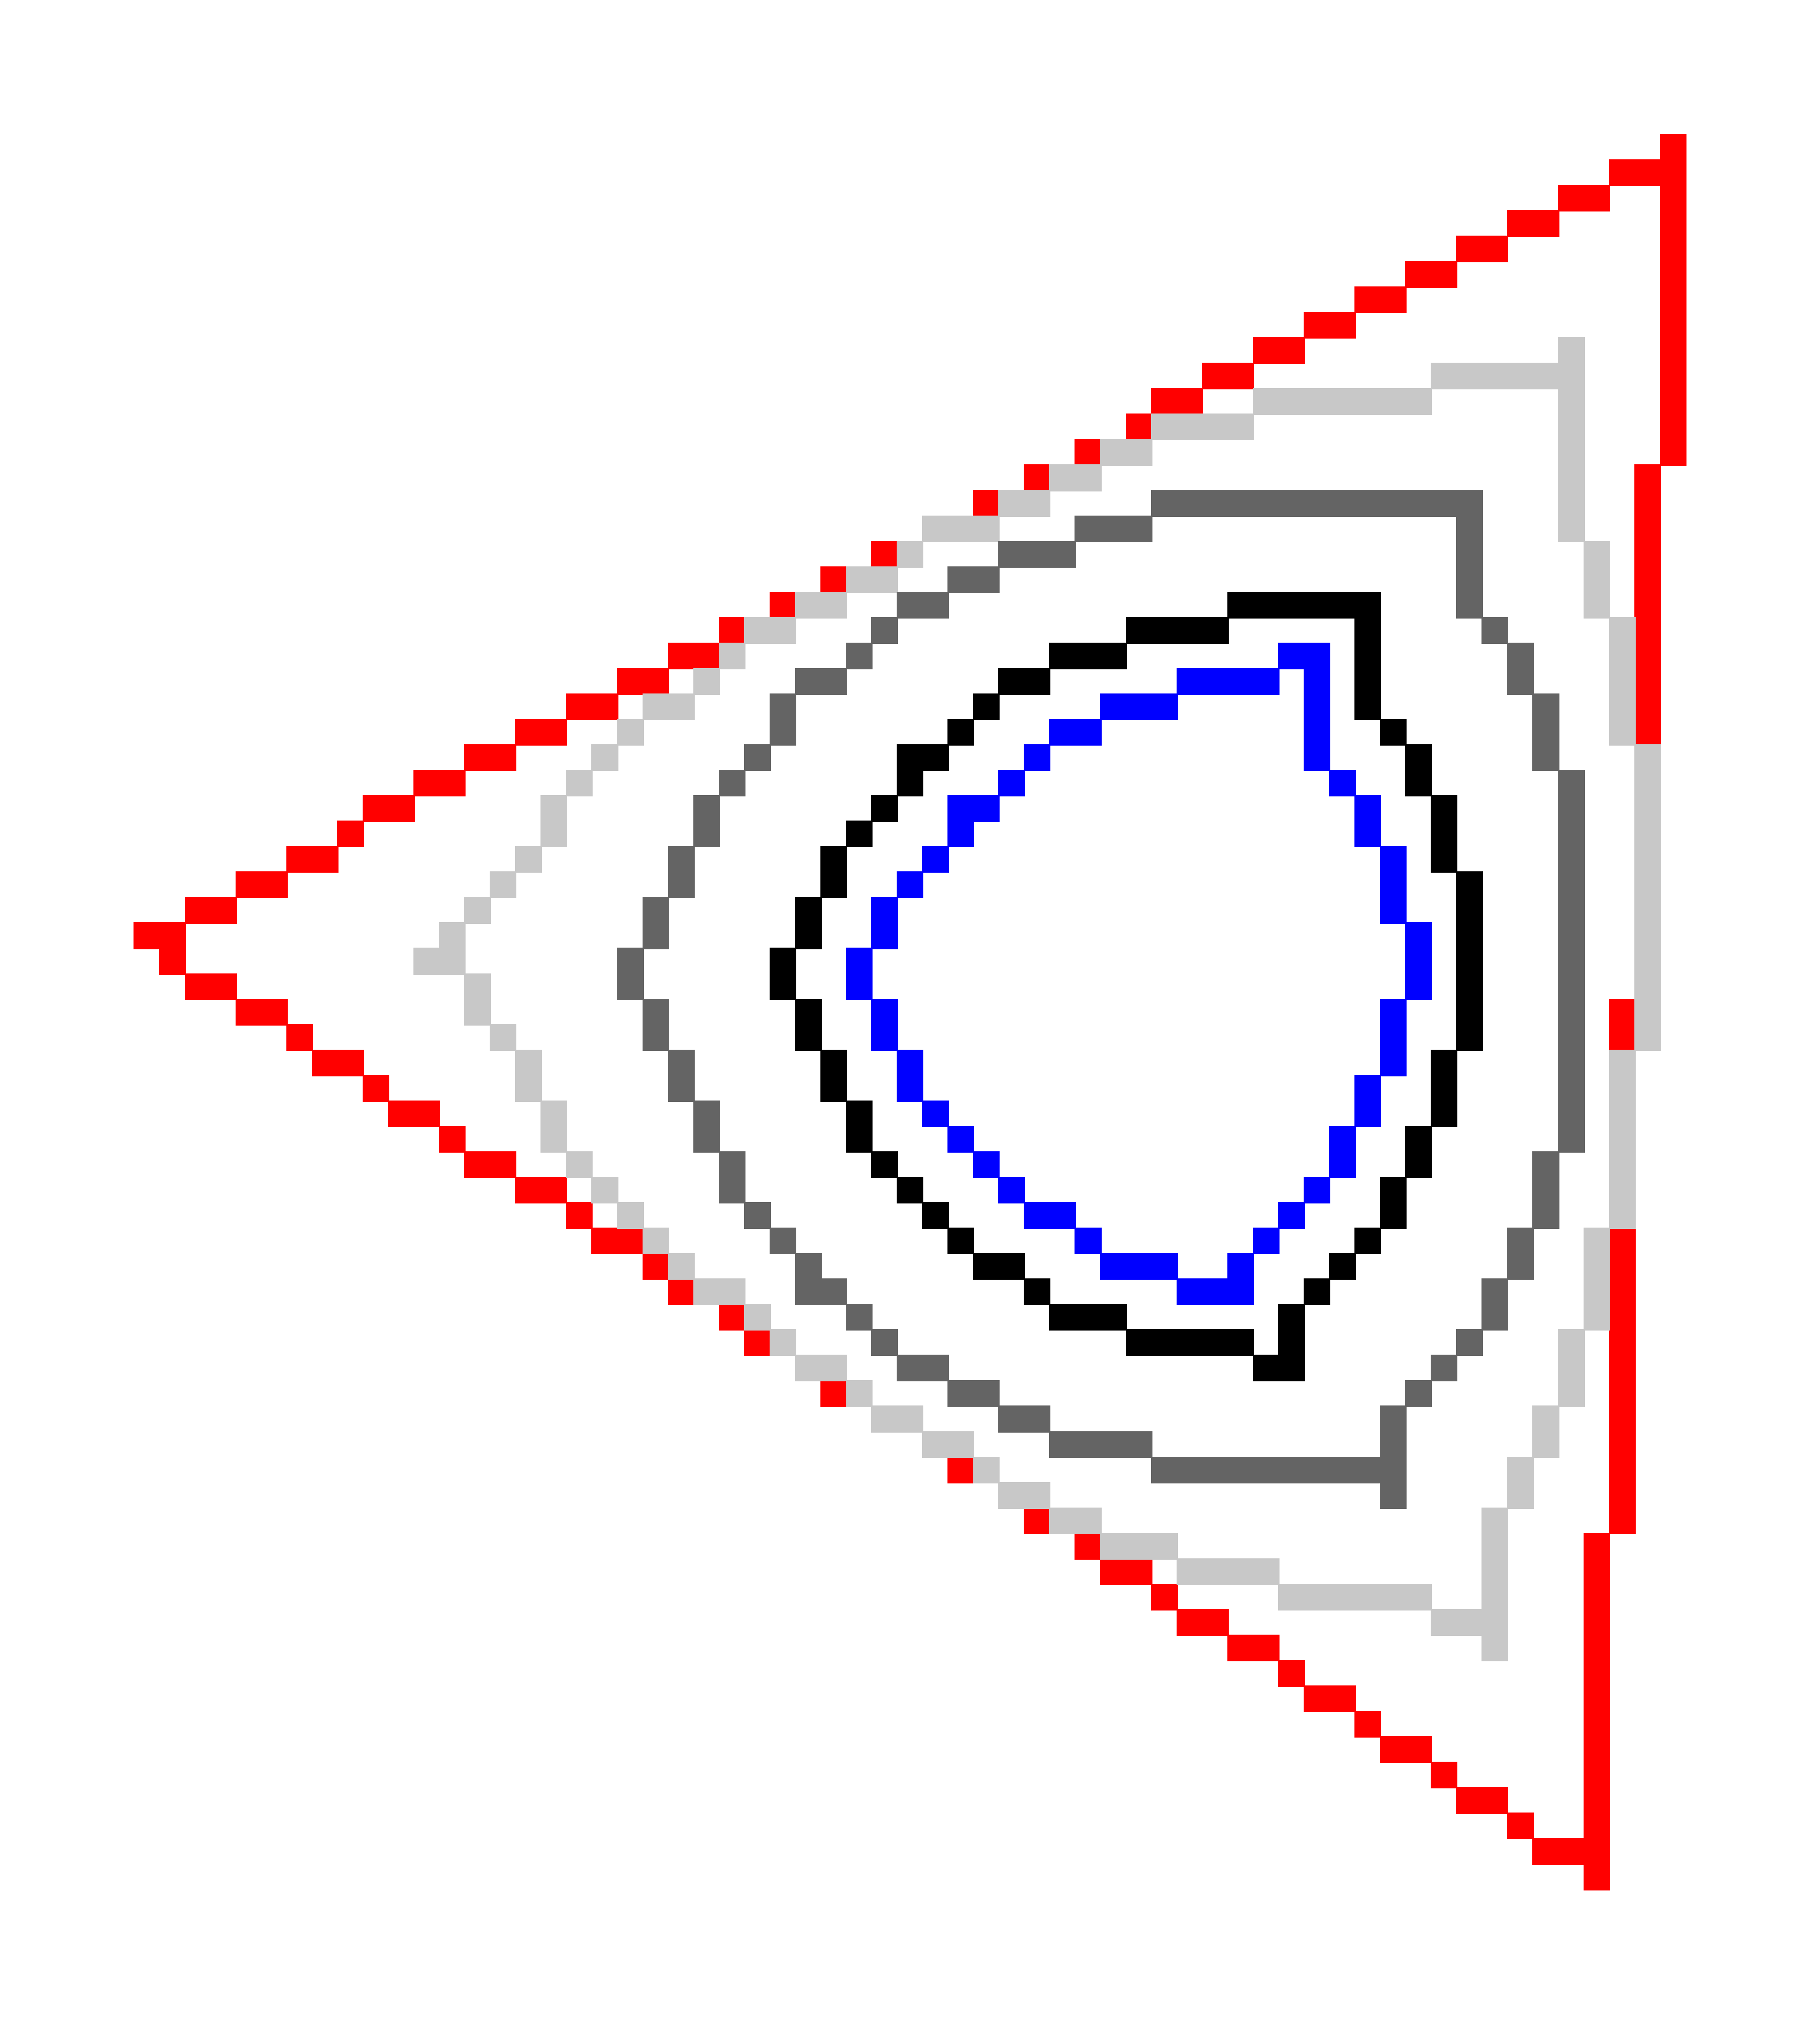
\includegraphics[scale=0.03]{images/flow-b10-ls10/Triangle.eps}}%
		\hspace{15pt}
		\subfloat{%

\includegraphics[scale=0.03]{images/flow-b10-ls10/Square.eps}}%		
		\hspace{15pt}
		\subfloat{%

\includegraphics[scale=0.025]{images/flow-b10-ls10/Flower.eps}}%
		}

		\setcounter{subfigure}{-1}			
		\subfloat[$r=5,\ell=5$ ($1.5\times$ scaling)]{
		\subfloat{%
		
\includegraphics[scale=0.016]{images/flow-b5-ls5-scaled/Ball.eps}
		}%
		\hspace{15pt}
		\subfloat{%
		
\includegraphics[scale=0.02]{images/flow-b5-ls5-scaled/Triangle.eps}}%
		\hspace{15pt}
		\subfloat{%

\includegraphics[scale=0.02]{images/flow-b5-ls5-scaled/Square.eps}}%		
		\hspace{15pt}
		\subfloat{%

\includegraphics[scale=0.016]{images/flow-b5-ls5-scaled/Flower.eps}}%
		}

		\caption{Digital curvature flow for four different shapes. A total of 20 iterations were executed for each flow, except for (c) (7 iterations). Curves are displayed every 2 iterations. The initial curve (countour of the original shape) is in red and the end curve in blue.}
		\label{fig:digital_flows}	
	\end{figure}


\begin{table}[!ht]
\center
\begin{tabular}{l|c|c|c|c}
	& \multicolumn{4}{c}{Digital Elastica}\\
	\hline
	& Ball & Triangle  & Square & Flower \\
	\hline
	Initial value & 0.156 & 2.55 & 1.81 & 4.196\\
	\hline	
	$\mathbf{r=3,\ell=3}$ & 0.192 & 0.335 & 0.286 & 0.298\\
	\hline
	$r=5,\ell=2$ & 0.156 & 0.556 & 0.423 & 1.477 \\
	$r=5,\ell=3$ & 0.166 & 0.375 & 0.321 & 0.364 \\	 
	$r=5,\ell=4$ & 0.207 & 0.508 & 0.311 & 0.174\\
	$\mathbf{r=5,\ell=5}$ & 0.193 & 0.52 & 0.278 & 0.163\\	
	\hline
	$\mathbf{r=10,\ell=10}$ & 0.216 & 1.33 & 0.333 & 0.159		
\end{tabular}
\caption{Evaluation of digital elastica ($\alpha=0$) for start and end curves of the flow. Except for the ball, all the elastica energies were decreased significantly.}
\label{tab:digital_glows_elastica_result}
\end{table}

\subsection{Optimization Method}\label{sec:optimization_method}

Let $F$ be a function of $n$ binary variables, i.e.

\begin{align*}
F(y_1,\cdots, y_n) = \sum_{i}{F_i(y_i)} + \sum_{i < j}{F_{i,j}(y_i,y_j)}
\end{align*}

Function $F$ is submodular if and only if the following inequality holds for each pairwise term $F_{i,j}$ \cite{kolmogorov04}

\begin{align*}
	\quad F_{i,j}(0,0) + F_{i,j}(1,1) \leq F_{i,j}(0,1) + F_{i,j}(1,0)
\end{align*}

Energy \eqref{eq:curvature_highlighting_simplified} is non-submodular and optimizing it is a difficult problem, which
constrained us to use heuristics and approximation algorithms. The QPBO method \cite{rother07} transforms the
original problem in a max-flow/min-cut formulation and returns a full optimal labeling for submodular energies. For
non-submodular energies the method is guaranteed to return a partial labeling with the property that the set of labeled
variables is part of an optimal solution. That property is called partial optimality.

In practice, QPBO can leave many pixels unlabeled. There exist two extensions of QPBO that ameliorate this limitation: QPBOI
(improve) and QPBOP (probe). The first is an approximation method that is guaranteed to not increase the energy, but we
lost the property of partial optimality. The second is an exact method which is reported to label more variables than
QPBO. We use QPBOP. The extended computation region also regularizes the energy and we have checked that it induces a
higher number of labeled variables.
	
\section{Application in Image Segmentation}

The digital curvature flow can be applied as a post-processing step in an image segmentation framework. We use graph cut
\cite{boykov01} as segmentation method and we execute the flow for $n$ iterations. We include the graph cut data
fidelity term $g$ and standard length penalization $s$ to the flow energy.



\begin{align}			
	\min_{Y} \sum_{y \in Y}{\left( \alpha \cdot s(y) + \gamma \cdot g(y) \right)} + \beta \cdot \sum_{p \in A}{\hat{\kappa}_{r}^2(p)}.
	\label{eq:boundary-correction-energy}
\end{align}
	
	Let $\mathcal{N}_4(p)$ denote the four neighborhood of pixel $p$. Length penalization is defined as
	\begin{align*}
		s(p)=\sum_{p_k \in \mathcal{N}_4(p)}{ (p-p_k) }^2.
	\end{align*}


        In Figure \ref{fig:butterfly_results} we show some results. The flow clearly regularizes the contour of figures
        produced by the comparison segmentation via graph cut. In both figures, the flow is able to correct zones of high positive
        curvature and expand regions of low negative curvature, but without invading the background zone. Nonetheless,
        the flow does not expand zones of convexity. Unfortunately, as we follow a local strategy, we are unable to expand
        some zones that clearly belongs to the segmented object, like the cow's leg.

\section{Conclusion}
We have shown that the integral invariant curvature estimator can be integrated into an optimization model and can be
applied together with classical penalization terms as length and data fidelity in an image processing task. We
demonstrated its potential by designing a digital curvature flow that mimics continuous flow in an accurate way. Finally, we show how it can be used as a post-processing tool in an image segmentation framework.

We have some directions for future work. First, optimize the code and evaluate a runtime analysis to compare with
competitor methods. We also think that we can reformulate the model in \cite{schoenemann09} using the digital estimator
$\hat{\kappa_r}$. %We are working to achieve results with a lower running time.
	
	\begin{figure}[!ht]
		\center
		\subfloat[\label{fig:butterfly_initial}]{%
			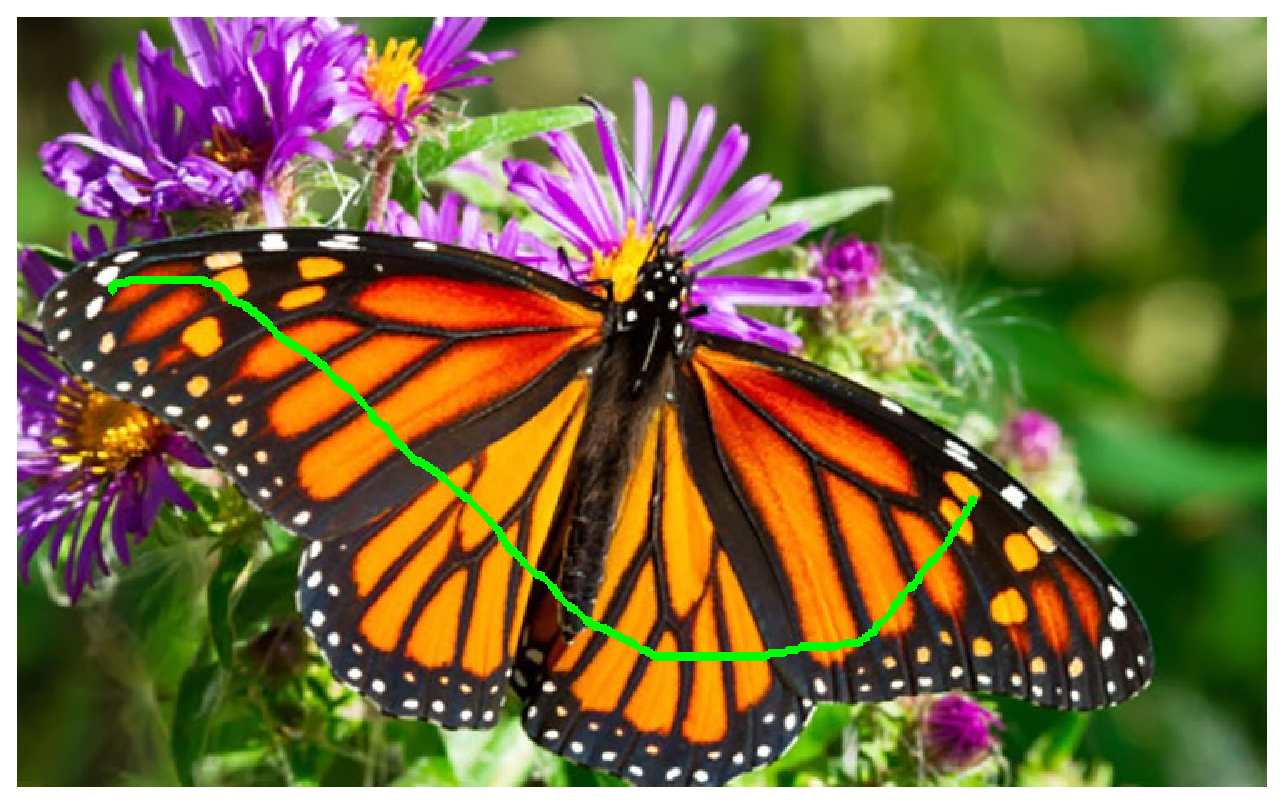
\includegraphics[scale=0.3]{images/butterfly/initial-seed.eps}
		}\hspace{10pt}%
		\subfloat[\label{fig:cow_initial}]{%
		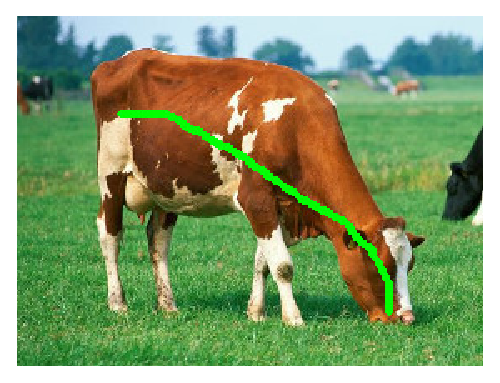
\includegraphics[scale=0.66]{images/cow/initial-mark.eps}
		}
		
		\begin{minipage}[b]{0.4\textwidth}
		\subfloat[\label{fig:butterfly_gc}]{%
		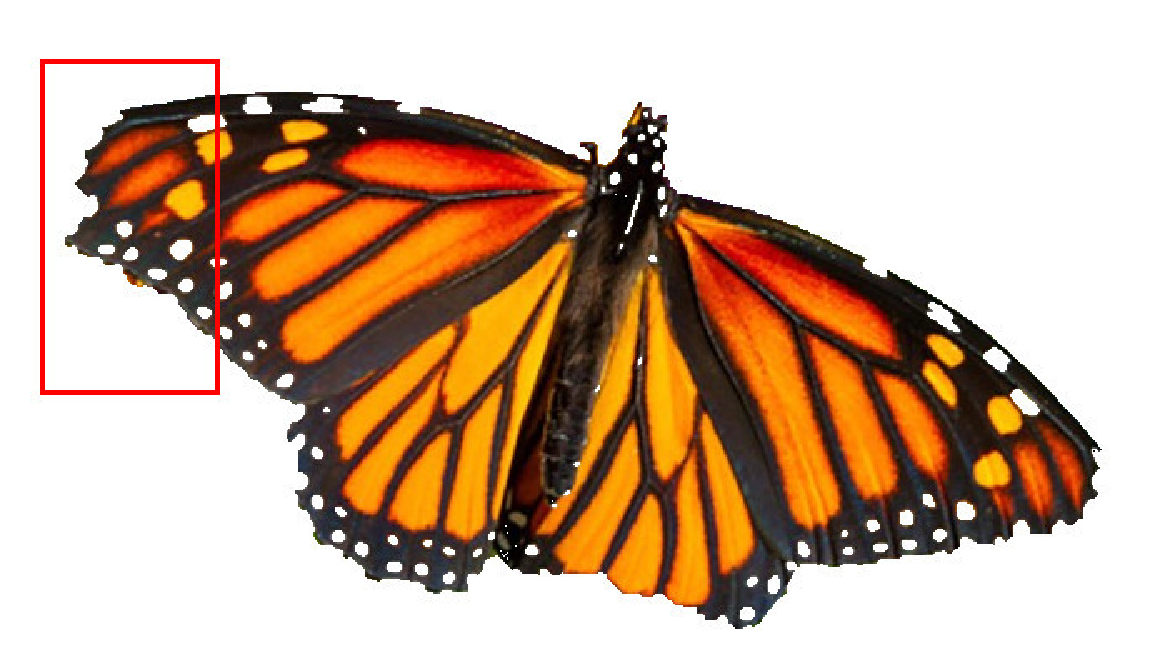
\includegraphics[scale=0.25]{images/butterfly/gc-marks.eps}
		}
		
		\subfloat[\label{fig:butterfly_cor}]{%
		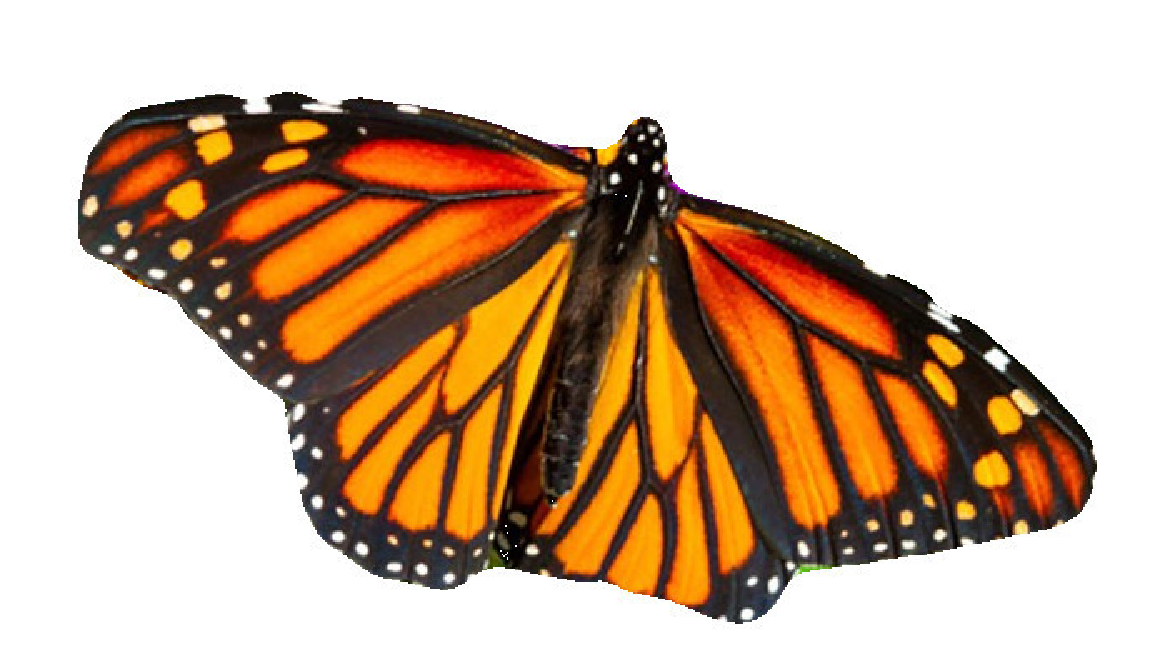
\includegraphics[scale=0.25]{images/butterfly/cor.eps}
		}%		
		\end{minipage}%
		\begin{minipage}[b]{0.6\textwidth}
		\center
		\subfloat[\label{fig:cow_gc}]{%
		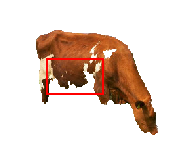
\includegraphics[scale=1.5]{images/cow/gc-marks.eps}
		}%
		\subfloat[\label{fig:cow_gc}]{%
		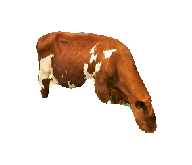
\includegraphics[scale=1.5]{images/cow/cor.eps}
		}%						
		\end{minipage}\vspace{1em}
								
		\begin{minipage}[b]{0.5\textwidth}
		\center
		\subfloat[\label{fig:butterfly_gc_m1}]{%
		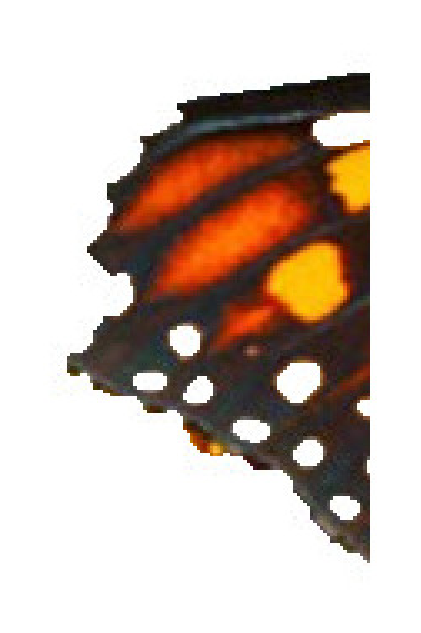
\includegraphics[scale=0.5]{images/butterfly/gc-mark-1.eps}
		}%
		\subfloat[\label{fig:butterfly_cor_gc1}]{%
		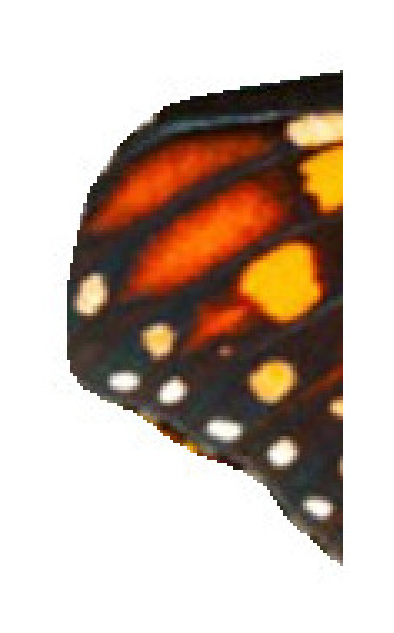
\includegraphics[scale=0.5]{images/butterfly/cor-mark-1.eps}
		}	
		\end{minipage}%		
		\begin{minipage}[b]{0.6\textwidth}
		\center
		\subfloat[\label{fig:cow_gc}]{%
		
\includegraphics[scale=4]{images/cow/gc-mark.eps}
		}
		
		\subfloat[\label{fig:cow_gc}]{%
		
\includegraphics[scale=4]{images/cow/cor-mark.eps}
		}%						
		\end{minipage}
				

		\caption{Digital flow post-processing results for a total of 5 iterations ($\alpha=0.1, \beta=1,\gamma=1$). }
		\label{fig:butterfly_results}
	\end{figure}%	


%
% ---- Bibliography ----
%
% BibTeX users should specify bibliography style 'splncs04'.
% References will then be sorted and formatted in the correct style.
%
\bibliographystyle{splncs04}
\bibliography{digital-curvature-boundary-correction}

\end{document}
